\section{Reinforcement Learning}
\begin{itemize}
	\item RL for ML4QS to learn from interactions with user and influencing him
	\item General overview of how to integrate RL in ML4QS is shown in Figure~\ref{fig:chapter_9_RL_loop}
	\begin{figure}[ht!]
		\centering
		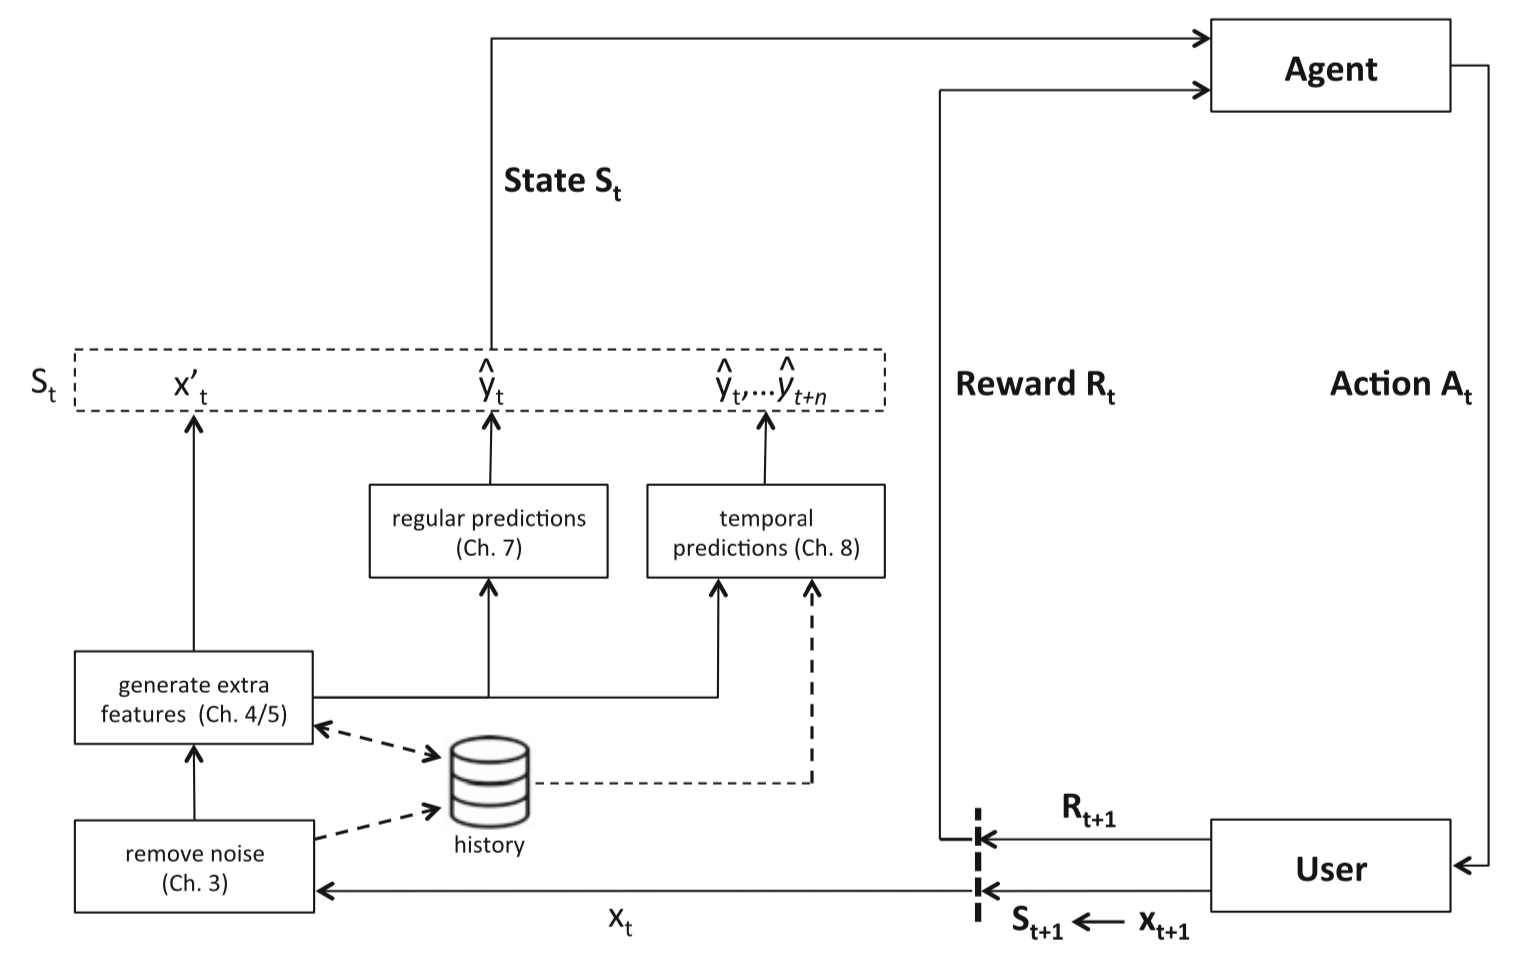
\includegraphics[width=0.5\textwidth]{figures/chapter_9_RL_loop.png}
		\caption{Reinforcement Learning in the loop for ML4QS}
		\label{fig:chapter_9_RL_loop}
	\end{figure}
	\item \textbf{Markov Property}: $\mathbb{P}\left\{R_{t+1}=r, S_{t+1}=s|S_0, A_0, R_0, ..., S_t, A_t, R_t\right\} = \mathbb{P}\left\{R_{t+1}=r, S_{t+1}=s|S_t, A_t\right\}$\\
	The conditional probabilities of future state and rewards solely depend on the last state $S_t, A_t$. 
	\item For every problem that satisfies this property, we can easily create a Markov Decision Process with a finite set of states as in Figure~\ref{fig:chapter_9_MDP}
	\begin{figure}[ht!]
		\centering
		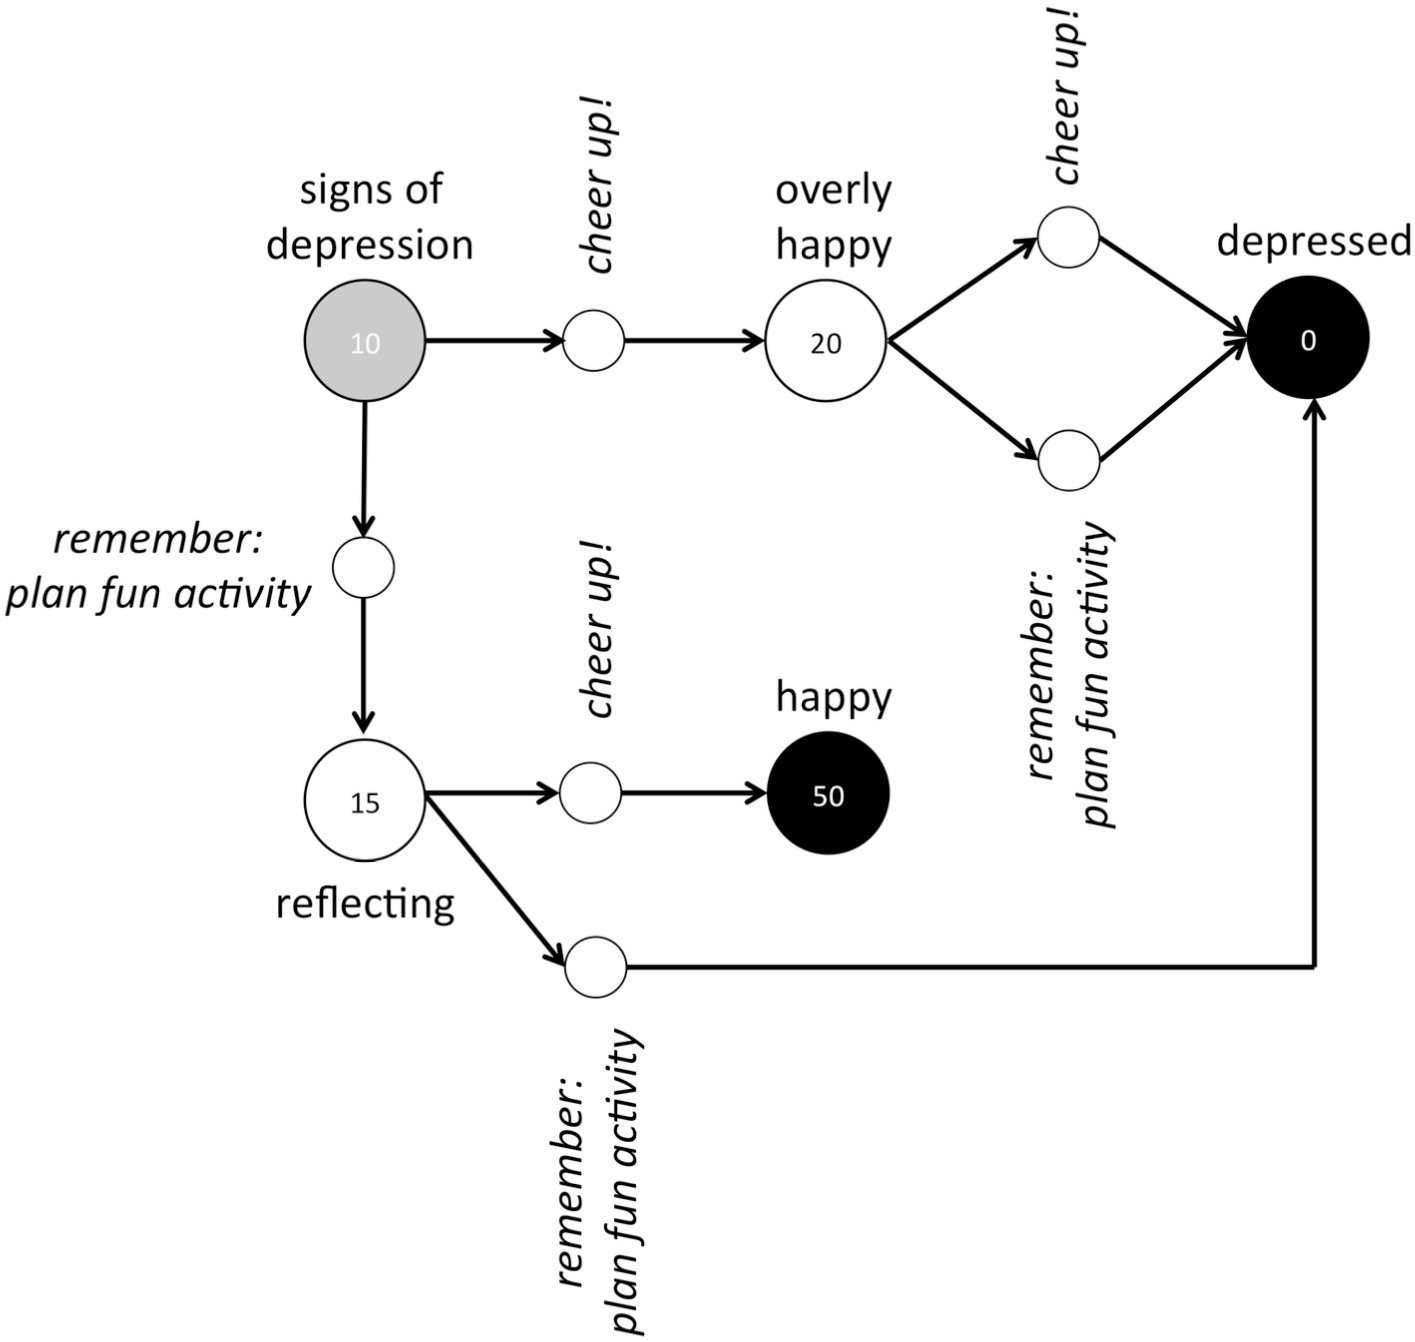
\includegraphics[width=0.35\textwidth]{figures/chapter_9_MDP.png}
		\caption{Markov Decision Process for simple example}
		\label{fig:chapter_9_MDP}
	\end{figure}
	\item \textbf{SARSA}:
	\begin{itemize}
		\item On-policy optimization, update $Q$-values by:
		$$Q(S_t, A_t) \leftarrow Q(S_t, A_t) + \alpha(R_{t+1} + \gamma Q(S_{t+1}, A_{t+1}) - Q(S_t, A_t))$$
		\item Popular policies are $\epsilon$-greedy or softmax over q-values for different actions
	\end{itemize}
	\item \textbf{Q-Learning}:
	\begin{itemize}
		\item Off-policy optimization, update by taking the maximum Q-value over next state:
		$$Q(S_t, A_t) \leftarrow Q(S_t, A_t) + \alpha(R_{t+1} + \gamma \max\limits_{A'(S_{t+1})} Q(S_{t+1}, A') - Q(S_t, A_t))$$
	\end{itemize}
	\item \textbf{Eligibility traces}: update frequently seen states in a single run more
	\begin{itemize}
		\item If we have seen a state and action combination more frequently in our history, then we want to increase the weight of the update because it is more eligible (i.e. more responsible for the outcome). We can determine the eligibility by:
		$$Z_t(s, a) = \begin{cases}
		\gamma \lambda Z_{t-1} + 1 & \text{if } s=S_t\wedge a=A_t\\
		 \gamma \lambda Z_{t-1} & \text{otherwise}
		\end{cases}$$
		\item In our learning algorithms, we can incorporate this by increasing the weight of the update, as e.g. in Q-Learning:
		$$Q(S_t, A_t) \leftarrow Q(S_t, A_t) + \alpha(R_{t+1} + \gamma \max\limits_{A'(S_{t+1})} Q(S_{t+1}, A') - Q(S_t, A_t))\cdot Z_t(s,a)$$
	\end{itemize}
	\item Usually, the Q-values are stored in a table. If the number of states and actions are very large, this is not feasible. Alternative is to learn a function/model, that takes as input the state and action, and predicts the Q-value.
	\item For continuous state spaces, we can discretize it by e.g. the \textbf{U-tree} algorithm
	\begin{itemize}
		\item Start with a single unit/leaf/discrete state where all continuous states are mapped to 
		\item Collect data by trial and error for a while and estimate the Q-values
		\item On the collected data for each leaf, we test whether we can find splits for any attribute $X_i$ with a significant difference in Q-values
		\item Choose $X_i$ and its split with the lowest $p$-value, and create new leafs. Continue until maximum number of leafs is reached
	\end{itemize}
\end{itemize}